\documentclass{article}
\usepackage{multirow}
\usepackage{subcaption}
\usepackage[labelformat=parens,labelsep=quad,skip=3pt]{caption}
\usepackage{graphicx}
\usepackage{textcomp}
\usepackage[ruled,vlined]{algorithm2e}

\title{Effective Text Augmentation strategy for NLP Models}


\begin{document}

\maketitle

\begin{abstract}
Data Augmentation is proved to be effective in Vision tasks. This paper proposes a strategy, through which training data can be increased in a meaningful way, and there by achieve good performance. This work tests four augmentation operations for transforming text (Random Swap, Random Deletion, Back-translation, Random Synonym Insertion) in two different settings on a classification model. Our paper proposes a mixed augmentation strategy which involves pre- and post- augmentation by leveraging all the four operations. Experimental results show that our method achieves a significant improvement on datasets of limited training data.

Keywords :  Data Augmentation, Natural Language Processing, sentiment analysis, Back translation, Random Swap, Random Deletion, Synonym Replacement.


\end{abstract}

 

\section{Introduction}
Nowadays, highly advanced applications in the filed of Natural Language Processing (NLP) are ubiquitous and it involves the computational processing and understanding of human languages. Incredible progress has taken place, particularly in the last few years in deep learning based NLP. The field of NLP is relied on statistics, probability, and machine learning since the 1980s, and on deep learning since 2010s\cite{otter2020survey}.  Machine Learning and Deep Learning have obtained significant results on the tasks ranging from Sentiment Analysis \cite{tang2015deep} to Question Answering \cite{malinowski2017ask}. 

Even though there are many advantages from deep learning, there are also more common challenges \cite{li2017deep} when it comes to NLP, because of the lack of theoretical foundation, lack of interpretability of the model, and the requirement of a huge amount of data and powerful computing resources. High performance of any model always depends on the size and quality of the data on which the model gets trained \cite{pepe2013testing}. Data Augmentation (DA) is a technique to increase the training data, it helps to boost the performance of the model. Image data augmentation is a standard practice in Computer Vision tasks and they performed remarkably well on many tasks \cite{perez2017effectiveness, shorten2019survey}, whereas Text data augmentation is rare in NLP tasks \cite{young2018recent}, due to the challenges it involves. The reasons for these challenges is coming up with rules for language transformation is not thoroughly studied and experimented. Few methods have already been proposed to increase the amount of training data using simple text transformations or text generation through language models \cite{abonizio2020pre}. Therefore, text data augmentation for NLP tasks becomes appealing.

In this work, we propose a text data augmentation strategy based on increasing training data before model training and augmenting the data while training the model. For implementing this strategy, we are adopting four text augmentation methods like Random Swap (RS), Random Deletion (RD), Back-translation(BT) and Random Synonym Insertion (RSI). The proposed strategy is evaluated on Apple Twitter Sentiment (ATS) Dataset\footnote{https://www.kaggle.com/c/apple-computers-twitter-sentiment2}, a dataset for sentiment classification. The results show that the proposed approach can obtain a significant improvement when the training data is limited.

The rest of the paper is organized as follows. Section 2 addresses the previous work happened in the text augmentation area. Section 3 skims through the adopted augmentation techniques, and how well they are working through pre and post augmentation strategies, and presents the proposed approach. Section 4 explains the experimental setup along with results and analysis and it is followed by Conclusion.


\section{Related Work}
Previous work has proposed some text augmentation techniques. A popular study called Back-translation, can generate new data by translating sentences from one languge to another and it is an effective method for Neural Machine Translation (NMT) to improve translation quality \cite{fadaee2018back}. Synonym identification and replacement \cite{anders2020dynamic} is another study carried out to transform sentences into another with similar meaning. Data noising is another approach studied for augmentation, it is widely adopted in application domains like vision and speech \cite{xie2017data}. Easy data augmentation (EDA)\cite{wei2019eda} proposed four techniques to do transformations in NLP, which includes synonym replacement, random insertion, random swap, and random deletion. EDA has shown significant performace improvement over text classification tasks.

In this paper, we are proposing an approach which augments the data before training and while training on batches. The proposed method follows a combination of RS, RD, BT, and RSI methods to perform text augmentaion. We evaluated the proposed method on a classfication task, and a significant improvement is achieved on a smaller dataset. Code is publicly available here\footnote{https://github.com/sridevibonthu/TextAugmentation}.


\section{Our Approach}
\subsection{Augmentation Techniques adopted}

\subsubsection{Random Swap (RS)}
This approach randomly selects two words and swaps them in a training example, $x$, and repeats this process for $n$ number of times to generate an augmented example, $\hat{x}$. Fig. \ref{fig:randomswap} illustrates this process with an example. 
\begin{equation}
\hat{x} = RandomSwap(x, n)
\end{equation}
This is a very simple approach to generate new training examples from the existing. Downside of this approach is it may cause adversarial text attack to fool the model especially if the sentence has nouns. For example "Rama Killed Ravana" is completely different from "Ravana killed Rama". This technique can be adopted based on the nature of the training examples.

\begin{figure}[h!]
\centering
  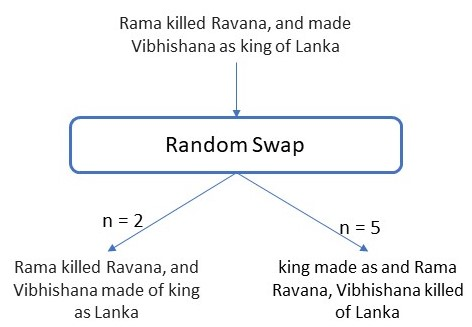
\includegraphics[width=0.6\textwidth]{randomswap.jpg}
  \caption{Random Swap operation generating two transformed examples from a single input $x$ for the $n$ values 2 and 5.}
  \label{fig:randomswap}
\end{figure}

\subsubsection{Random Deletion (RD)}
This approach randomly deletes $n$ number of words from the training example, $x$ with a probability $p$ and generates an augmented training example $\hat{x}$. A sample example is shown in Fig. \ref{fig:randomdelete}. If the value of $p$ is large, then it may result in meaningless sentences and sometimes the context may change completely.
\begin{equation}
\hat{x} = RandomDeletion(x, p)
\end{equation}
\begin{figure}[h!]
\centering
  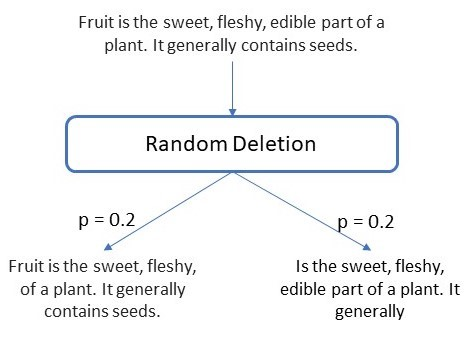
\includegraphics[width=0.6\textwidth]{randomdelete.jpg}
  \caption{Random Deletion operation generating two transformed examples for a single input $x$, with a common probability value of $0.2$.}
  \label{fig:randomdelete}
\end{figure}

\subsubsection{Back Translate (BT)}
This approach translates a training example, $x$ from source language($SL$) to some intermediate language ($IL$), and again back-translates it to source language. This technique generates synthetic data in four lines of code, but this is computationally expensive as it has to do language translation twice back to back. Fig. \ref{fig:backtranslate} shows two examples in which German and French are chosen as intermediate languages for translation.
\begin{equation}
\hat{x} = translate( translate(x, SL, IL), IL, SL)
\end{equation}
\begin{figure}[h!]
\centering
  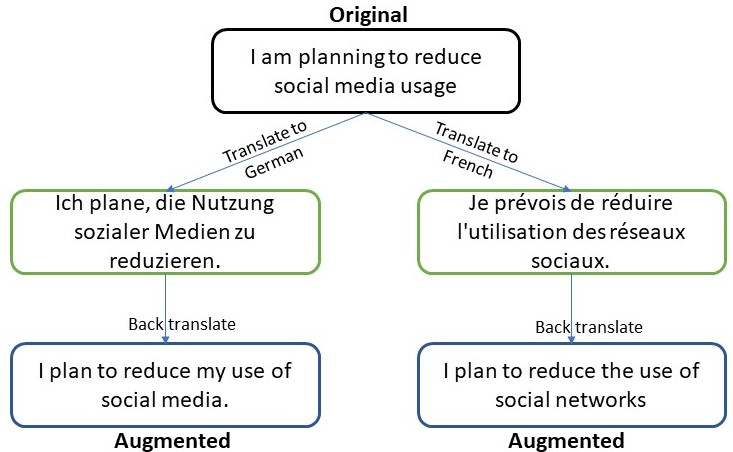
\includegraphics[width=0.8\textwidth]{backtranslate.jpg}
  \caption{Back-translation operation generating two augmented examples for the same input, $x$, by taking two intermediate languages.}
  \label{fig:backtranslate}
\end{figure}

\subsubsection{Random Synonym Insertion (RSI)}
This approach randomly inserts synonyms of of $n$ words, which are not stop-words in a training example, $x$ to generate a new training example, $\hat{x}$. An example for Random Insertion with Synonym is shown in Fig. \ref{fig:randominsert}. The outcome of this technique depends on the value of $n$. The suggestible value for $n$ can be in the range of 1 to 3. 
\begin{equation}
\hat{x} = RandomInsertion(x, n)
\end{equation}

\begin{figure}[h!]
\centering
  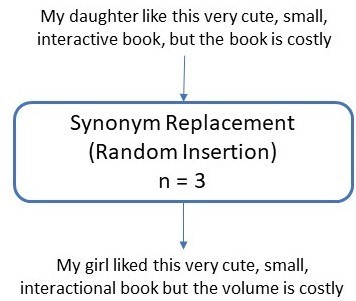
\includegraphics[width=0.6\textwidth]{random insertion.jpg}
  \caption{Random Insertion operation generating an augmented example in which \textit{(daughter, interactive, book)} are replaced with \textit{(girl, interactional, volume)}.}
  \label{fig:randominsert}
\end{figure}

Random Insertion technique with synonym replacement can generate a new training example but it suffers with a deficiency. This may cause adversarial text attack as shown below.

\textbf{input x} \textrightarrow \textit{"True Grit" was the best movie I have seen since I was a small boy.} (Predicted as positive)

\textbf{Random Insertion(x, n = 2 ) = Augmented $\hat{x}$} \textrightarrow \textit{"True Grit" was the best movie I have seen since I was a \textbf{wee lad}}. {predicted as negative}


\subsection{The Classification Model}	

A text classification problem can be defined as a set of training examples $D = \{ x_1, x_2, . . ., x_N\}$ in which every record is labelled with a class value drawn from a set of discrete class labels indexed by ${1..k}$ \cite{aggarwal2012survey}. The classification model is constructed based on the training examples, and evaluated with the test set. Our paper used Recurrent Neural Network (RNN) language model based on Long Short Term Memory Network (LSTM) \cite{can2018multilingual}. LSTM is better in analyzing emotion of long sentences and it is applied to achieve multi-classification for text emotional attributes \cite{li2016text}. This model is applied on  the Apple Twitter Sentiment Dataset\footnote{https://www.kaggle.com/c/apple-computers-twitter-sentiment2} to study the effectiveness of the selected text augmentation techniques in both the approaches and to come up with a best strategy for augmentation.

The LSTM-RNN takes in a training example as a sequence of words, $X = {x_1, x_2, .., x_T}$ one a time and produces cell state, $c$, and hidden state, $h$, for each word. The network is used recurrently by feeding the current word $x_t$, cell state, $c$ and hidden state, $h$ from the previous word $(c_{t-1}, h_{t-1})$, to produce the next cell and hidden states, $(c_t, h_t)$. The final hidden state, $h_T$ obtained by sending last word in the sentence, $x_T$ to the LSTM cell is fed through a linear layer $f$ to get the predicted sentiment $\hat{y}$.
\begin{equation}
(c_t, h_t) = LSTM (x_t, h_{t-1}, c_{t-1}) 
\end{equation}
\begin{equation}
\hat{y} = f(h_T)
\end{equation}

\subsection{Evaluation of Augmentation Methods}
The simple LSTM classification model is trained without applying any augmentation on the original data and received a baseline accuracy of $72.75\%$. Each of the four augmentation strategies (RS, RD, BT, RSI) were evaluated on the Apple Twitter Sentiment Dataset individually by following two approaches to understand how they are performing. 

\begin{figure}
  \begin{subfigure}{6cm}
    \centering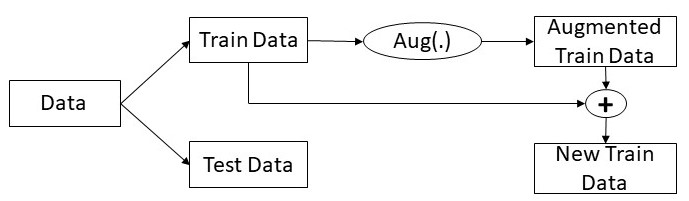
\includegraphics[width=5cm]{approach1.jpg}
    \caption{Pre-Augmentation}
  \end{subfigure}
  \begin{subfigure}{6cm}
    \centering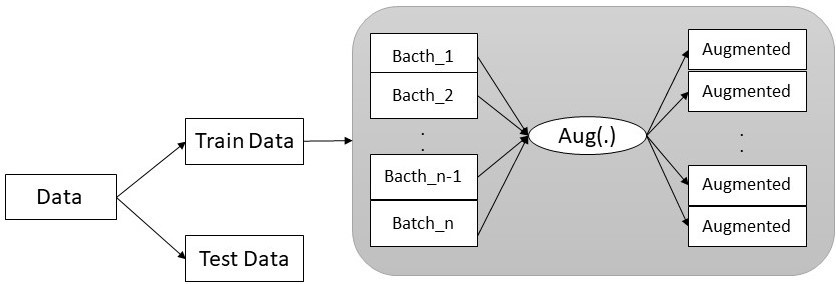
\includegraphics[width=5cm]{approach2.jpg}
    \caption{Post-Augmentation}
  \end{subfigure}
  \caption{Initial methods to test the adopted text augmentation strategies. (a) Approach 1 - pre-augmentation, which increases a fraction of training data. (b) Approach 2 - post-augmentation, which augments the data in the mini-batches while training.}
  \label{fig:initialmethods}
\end{figure}

\subsubsection{Approach - 1 ( Pre-augmentation )}
In the first approach the train set is increased by taking a fraction of the training examples, transforming using one of the augmentation technique from RS, RD, BT, and RSI (Fig. \ref{fig:initialmethods} ). Let $D : \{(x_i, y_i)\}_{i=1}^M$ is a set of $M$ training examples.
\begin{equation}
D_{New} = D + D_{Aug}
\end{equation}
\begin{equation}
D_{Aug} = T(\{(x_i, y_i)\}_{i=1}^{f.M})
\end{equation}
Where, $T$ is a transformation function, which augments a fraction, $f$ of the $M$ training samples to form new Training set, $D_{New}$. The new training set will $(1+f).M$ records after augmentation. This approach is followed for all the adopted augmentation techniques and all the methods improved the validation accuracy by 2 to 3\% when compared with baseline. Fig. \ref{fig:initialmethods} depicts the training accuracy vs. validation accuracy for all these four experiments and it is very clear that Back translation consistently maintained good validation accuracy when compared with baseline accuracy.

\subsubsection{Approach - 2 (Post-augmentation)}
In the second approach the training samples in a mini-batch set at $t^{th}$ training iteration, $D_t : \{(x_i, y_i)\}_{i=1}^M$  can be changed to $\hat{D_t} : \{(\hat{x_i}, y_i)\}_{i=1}^M$, by applying the augmentation techniques when they are fed into the LSTM network (Fig. \ref{fig:initialmethods}). This process repeats for every batch of every epoch of the training process. In this approach, the model encounters plenty of augmented training examples. 
Let $e$ be the number of epochs, and $b$ be the number of batches and $m$, the number of training samples in every batch, and if the augmentation happens randomly for 50\% of the training samples, then the overall augmented training samples seen by the model in the training phase are $e * b * (0.5 * m)$.

The augmentation techniques adopted to test this approach are RS and RD only. The reason for not adopting BT, RSI is they can work in sentence level, but not on token level, and in training the sentence is available in numerical format only. Fig. \ref{fig:postaugmentA2} depicts the training accuracy vs. validation accuracy for these two experiments. Both the methods helped improve validation accuracy, and Random Deletion also reduced overfitting.

\subsection{Proposed Approach}
By examining the performance of the text augmentation techniques adopted in the above two approaches, we have come up with a mixed augmentation startegy, in which a fraction of the original training data is transformed by using RS, RD, BT, RSI by following a randomized algorithm called \textit{pre-Augmentation(x)} and again randomly applying transformation on batches by using RS and RD by following \textit{post-Augmentation(x)} algorithm. In this approach, Fig. \ref{fig:proposedapproach}, there is a chance to apply augmentation on the augmented text i.e, Random Swap operation may happen on the back-translated text.

\begin{figure}[h!]
\centering
  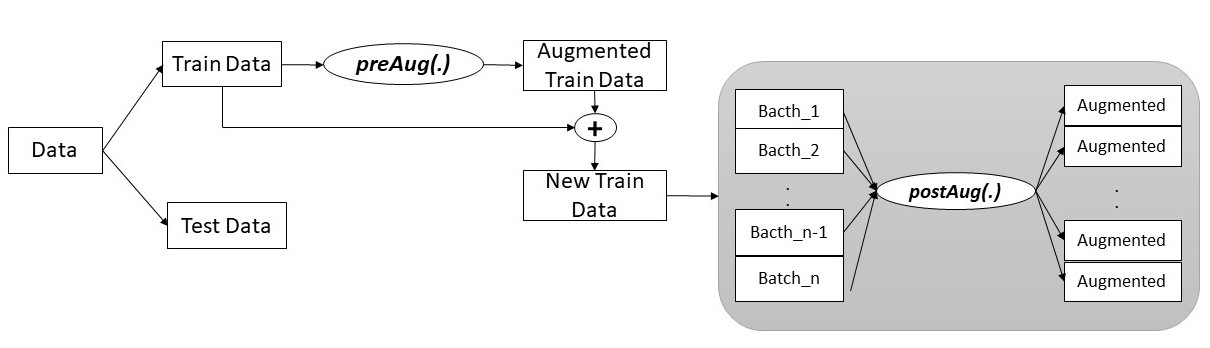
\includegraphics[width=0.8\textwidth]{proposedmethod.jpg}
  \caption{proposed method. Augmentation happens twice with preAug(.) and postAug(.) methods.}
  \label{fig:proposedapproach}
\end{figure}

\begin{algorithm}[H]
\SetAlgoLined
\KwResult{Transformed Exampmle $\hat{x}$ for the Training Example $x$}
rate := getRandom(0,1) \tcp*{returns a number between 0 and 1}
\eIf{ rate $<$ 0.3}{
$\hat{x} = RandomInsertion(x, n)$ \;
}{
\eIf{rate $<$ 0.6} {
$\hat{x} = translate( translate(x, SL, IL), IL, SL)$ \;
}
{
\eIf{rate $<$ 0.8}{
$\hat{x} = RandomDeletion(x, p)$ \;}
{
$\hat{x} = RandomSwap(x, n)$ \;}
}
}
\caption{Pre-Augmentation($x$)}
\end{algorithm}


\begin{algorithm}[H]
\SetAlgoLined
\KwResult{Transformed Exampmle $\hat{x}$ for the Training Example $x$}
rate := getRandom(0,1)    \tcp*{returns a number between 0 and 1}
\eIf{ rate $<$ 0.2}{
$\hat{x} = RandomSwap(x, n)$  \;
}{
\eIf{rate $<$ 0.6} {
$\hat{x} = RandomDeletion(x, p)$ \;
}
{
$\hat{x} = x$
}
}
\caption{Post-Augmentation($x$)}
\end{algorithm}

\section{Experiment}
\begin{figure}
  \begin{subfigure}{6cm}
    \centering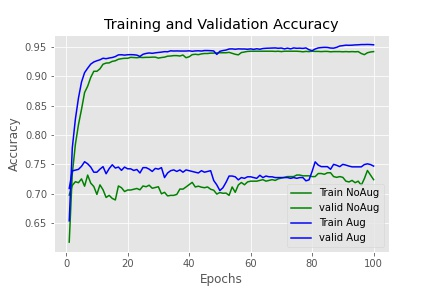
\includegraphics[width=5cm]{accuracyrandomswapA1.jpg}
    \caption{Random Swap}
  \end{subfigure}
  \begin{subfigure}{6cm}
    \centering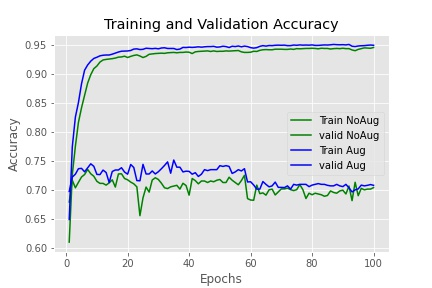
\includegraphics[width=5cm]{accuracyrandomdeleteA1.jpg}
    \caption{Random Deletion}
  \end{subfigure}
 
  \begin{subfigure}{6cm}
    \centering
\includegraphics[width=5cm]{accuracybacktranslate.jpg}
    \caption{Back translation}
  \end{subfigure}
  \begin{subfigure}{6cm}
    \centering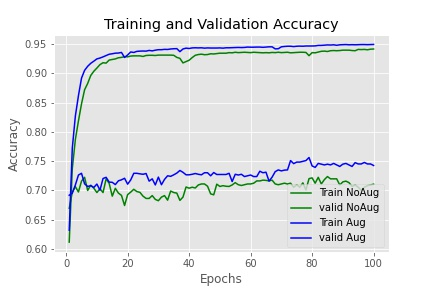
\includegraphics[width=5cm]{accuracyrandomInsertionA1.jpg}
    \caption{Random Synonym Insertion}
  \end{subfigure}
  \caption{Training vs. Validation accuracy by following Approach 1 (pre-augmentation) with RS, RD, BT, RSI.}
  \label{fig:preaugmentA1}
\end{figure}


\begin{figure}
  \begin{subfigure}{6cm}
    \centering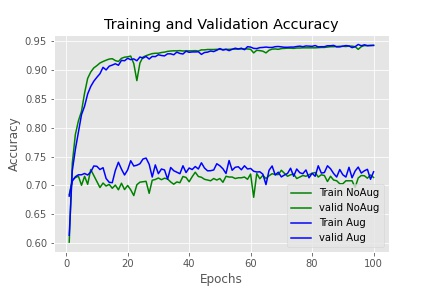
\includegraphics[width=5cm]{accuracyrandomswapA2.jpg}
    \caption{Random Swap}
  \end{subfigure}
  \begin{subfigure}{6cm}
    \centering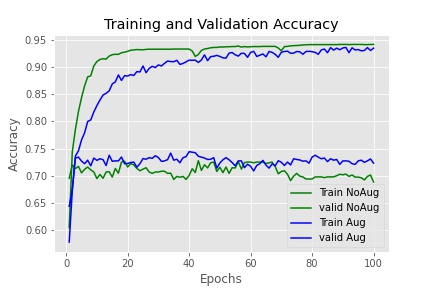
\includegraphics[width=5cm]{accuracyrandomdeleteA2.jpg}
    \caption{Random Deletion}
  \end{subfigure}
  \caption{Training vs. Validation accuracy by following Approach 2 (post-augmentation) with RS, RD.}
  \label{fig:postaugmentA2}
\end{figure}


\subsection{Data}
The Apple Twitter Sentiment dataset provided by kaggle for a competition called inclass prediction is utilized to carry out the experimentation. This dataset is suitable for the experiment because, testing proposed augmentation strategy needs to be evaluated in limited data settings. ATS dataset contains 3886 records in which 82 are not relevant. The tweets can be either positive, negative or neutral. The original training records we adopted for experimentation with class labels were provided in the bar chart at Fig. \ref{fig:dataset}. 80\% of the data is taken as training data and the rest as validation data to perform the experiment. \textit{ \\@ mentions, \#hashtag, RT (Retweet), hyperlinks} were removed as part of preprocessing the data, as the adopted data is from twitter.


\begin{figure}[h!]
\centering
  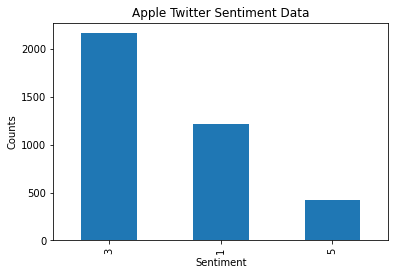
\includegraphics[width=0.7\textwidth]{dataset.png}
  \caption{Class-wise training examples in ATS Dataset (1 - Negative, 3 - Neutral, 5 - Positive)}
  \label{fig:dataset}
\end{figure}

\subsection{Experimental Setup}
The Data was tokenized with the help of \textit{spacy}\cite{srinivasa2018natural} tokenizer. \textit{TorchText}\footnote{https://pytorch.org/text/stable/index.html} library is utilized to complete the work. This library is part of PyTorch project, which contains data processing utilities and popular datasets for Natural Language Processing. 

A simple classification model based on LSTM is adopted and same hyper-parameters are used for all the \textbf{8} experimentations, baseline without augmentations(1), preaugmentation approach (Fig. \ref{fig:initialmethods}) for RS, RD, BT, RSI techniques (4), postaugmentation on batches (Fig. \ref{fig:initialmethods}) approach for RS, RD techniques(2) and for the proposed approach (Fig.\ref{fig:proposedapproach})(1). The dimension of word embeddings is 300 and the number of hidden units is 100. Dropout rate is 0.25 and the batch size is 32. Adam optimizer is used with an inital learning rate of 0.001. All training consists of 100 epochs. We report accuracy of all the experiments.

\subsection{Results and Analysis}
The resultant accuracies obtained by applying a single augmentation strategy from the set of RS, RD, BT, RSI in the approaches mentioned above are present in Table 1. RS and RSI have performed well if training data is increased before training, RD reduced the overfitting if the data is augmented while training on batches. Based on these observations Algorithm1 pre-augmentation(x), which randomly chooses one of the four techniques is used to increase the training data before training and Algorithm 2 post-augmentation(x), which randomly chooses either RS or RD while training were adopted as shown in Fig. \ref{fig:proposedapproach}. This approach has resulted with 76.05\%, which is an increase of +3.29, when compared with the baseline. The proposed approach outperformed all the simple approaches to augment the data for performance boosting. 

\begin{table}[]
\begin{tabular}{|c|l|l|l|l|}
\hline
\textbf{\begin{tabular}[c]{@{}c@{}}Augmentation\\ Strategy\end{tabular}} & \multicolumn{2}{c|}{\textbf{\begin{tabular}[c]{@{}c@{}}Approach - 1\\ pre-augmentation\end{tabular}}} & \multicolumn{2}{c|}{\textbf{\begin{tabular}[c]{@{}c@{}}Approach - 2\\ post-augmentation\end{tabular}}} \\ \hline
\textbf{RS}                                                              & 75.45                                             & + 2.7                                             & 74.74                                             & + 1.99                                             \\ \hline
\textbf{RD}                                                              & 75.15                                             & + 2.4                                             & 74.41                                             & + 1.66                                             \\ \hline
\textbf{BT}                                                              & 74.74                                             & + 1.99                                            &                                                   &                                                    \\ \hline
\textbf{RSI}                                                             & 75.51                                             & + 2.76                                            &                                                   &                                                    \\ \hline
\end{tabular}
\caption{Comparison of adopted augmentation techniques with a baseline accuracy of 72.75\%}
\end{table}

\begin{figure}[h!]
\centering
  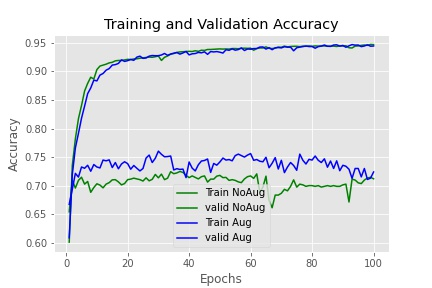
\includegraphics[width=0.8\textwidth]{accuracyproposed.jpg}
  \caption{Training vs. Validation accuracy of proposed approach.}
  \label{fig:accuracyproposed}
\end{figure}
\section{Conclusion}
This paper proposes a new data augmentation policy to increase the data before training and while training. Four augmentation methods, viz., Random Swap, Random Deletion, Back-translation and Random Synonym Insertion are chosen in such a way that all are contributing for performance boosting. The proposed approach achieves a significant improvement in the accuracy and also reduced overfitting. This approach is best suitable when the training data is limited and it can be easily adopted to any task and dataset. This augmentation strategy can be further fine-tuned based on the increase or decrease in loss while training.
\section{Acknowledgement}
This paper and the research behind it would not have been possible without the exceptional support and computing facilities of my Institution, Vishnu Institute of Technology.
\begin{thebibliography}{10}

\bibitem{otter2020survey} Otter, Daniel W., Julian R. Medina, and Jugal K. Kalita. "A survey of the usages of deep learning for natural language processing." IEEE Transactions on Neural Networks and Learning Systems (2020).

\bibitem{tang2015deep} Tang, Duyu, Bing Qin, and Ting Liu. "Deep learning for sentiment analysis: successful approaches and future challenges." Wiley Interdisciplinary Reviews: Data Mining and Knowledge Discovery 5.6 (2015): 292-303.

\bibitem{malinowski2017ask} Malinowski, Mateusz, Marcus Rohrbach, and Mario Fritz. "Ask your neurons: A deep learning approach to visual question answering." International Journal of Computer Vision 125.1-3 (2017): 110-135.


\bibitem{li2017deep} Li, Hang. "Deep learning for natural language processing: advantages and challenges." National Science Review (2017).

\bibitem{pepe2013testing} Pepe, Margaret Sullivan, et al. "Testing for improvement in prediction model performance." Statistics in medicine 32.9 (2013): 1467-1482.

\bibitem{perez2017effectiveness} Perez, Luis, and Jason Wang. "The effectiveness of data augmentation in image classification using deep learning." arXiv preprint arXiv:1712.04621 (2017).

\bibitem{shorten2019survey} Shorten, Connor, and Taghi M. Khoshgoftaar. "A survey on image data augmentation for deep learning." Journal of Big Data 6.1 (2019): 60.

\bibitem{young2018recent} Young, Tom, et al. "Recent trends in deep learning based natural language processing." ieee Computational intelligenCe magazine 13.3 (2018): 55-75.


\bibitem{young2018recent} Young, Tom, et al. "Recent trends in deep learning based natural language processing." ieee Computational intelligenCe magazine 13.3 (2018): 55-75.

\bibitem{abonizio2020pre} Abonizio, Hugo Queiroz, and Sylvio Barbon Junior. "Pre-trained Data Augmentation for Text Classification." Brazilian Conference on Intelligent Systems. Springer, Cham, 2020.

\bibitem{fadaee2018back} Fadaee, Marzieh, and Christof Monz. "Back-translation sampling by targeting difficult words in neural machine translation." arXiv preprint arXiv:1808.09006 (2018).

\bibitem{anders2020dynamic} Anders, Kelley L., et al. "Dynamic homophone/synonym identification and replacement for natural language processing." U.S. Patent No. 10,657,327. 19 May 2020.

\bibitem{xie2017data} Xie, Ziang, et al. "Data noising as smoothing in neural network language models." arXiv preprint arXiv:1703.02573 (2017).

\bibitem{wei2019eda} Wei, Jason, and Kai Zou. "Eda: Easy data augmentation techniques for boosting performance on text classification tasks." arXiv preprint arXiv:1901.11196 (2019).

\bibitem{aggarwal2012survey} Aggarwal, Charu C., and ChengXiang Zhai. "A survey of text classification algorithms." Mining text data. Springer, Boston, MA, 2012. 163-222.

\bibitem{can2018multilingual} Can, Ethem F., Aysu Ezen-Can, and Fazli Can. "Multilingual sentiment analysis: An RNN-based framework for limited data." arXiv preprint arXiv:1806.04511 (2018).

\bibitem{li2016text} Li, Dan, and Jiang Qian. "Text sentiment analysis based on long short-term memory." 2016 First IEEE International Conference on Computer Communication and the Internet (ICCCI). IEEE, 2016.

\bibitem{srinivasa2018natural} Srinivasa-Desikan, Bhargav. Natural Language Processing and Computational Linguistics: A practical guide to text analysis with Python, Gensim, spaCy, and Keras. Packt Publishing Ltd, 2018.


\end{thebibliography}
\end{document}